\chapter{Animationen}

\section{Motion Capture Aufnahmen}
Alle eingebundenen Animationen wurden zuvor von den Projektmitgliedern mit dem Motion Capture System im Keller der Hochschule Trier aufgenommen. Nachdem eine "uberschaubare Anzahl an qualitativ hochwertigen Aufnahmen ausgew"ahlt wurden, gingen diese direkt als .bvh Format zur Weiterverarbeitung.

\section{Einbindung der Animationen}
Die Einbindung der Animationen wurde wie das Modelling ebenfalls direkt in Blender vorgenommen. Mithilfe des Add-Ons ``MakeWalk`` ist es einfach, falls der selbst erstellte Rig keine Fehler aufweist, die rohen Motion Capturing aufnahmen in die 3D Software zu "ubertragen. F"ur jede Charakterklasse im Spiel wurde eine eigene ``Pose Libraries`` erstellt. Diese erwiesen sich durch einen strukturiertere und "ubersichtlichere Importierung in Unity als "au"sserst n"utzlich.\newline

Diese Animationen wurden in Unity importiert, und mit Hilfe eines Animators in eine Animation State Machine "uberf"uhrt, die je nach gew"ahlter Aktion und aktueller Haltung (Einh"andige Waffe, Zweih"andige Waffe, Nahkampfwaffe, Einsatzschild) , die korrekte Animation ausw"ahlt und abspielt.

Zus"atzlich wurden an einige der Animationen an bestimmten Zeitpunkten in der Animationen Funktionen angeh"angt. Somit kann erreicht werden, dass beispielsweise der Schusssound zum korrekten Zeitpunkt ausgel"ost wird, oder die Granaten im entsprechenden Frame erstellt, oder geworfen werden.

\begin{figure}
	\centering
	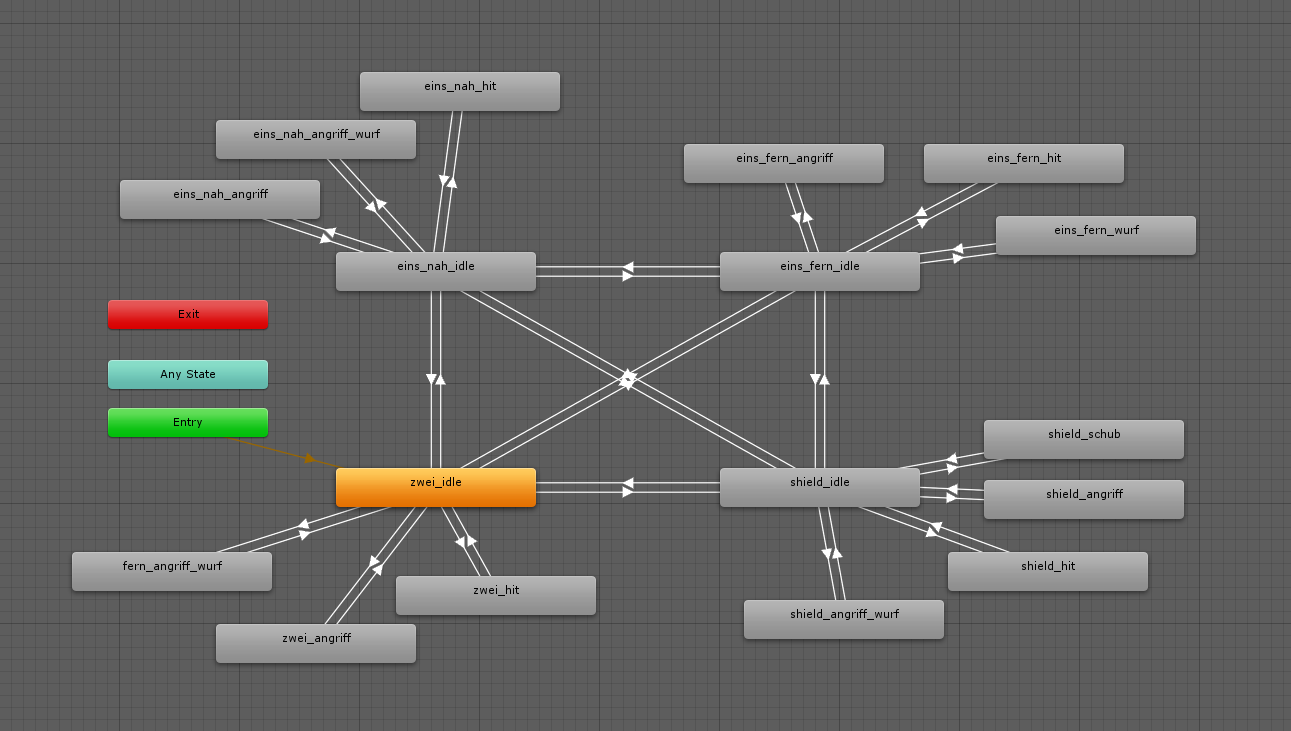
\includegraphics[height=9cm]{images/animator_tree.png}
	\caption{Animation Tree der Polizei Charaktere}
	\label{fig:anim_tree_police}
\end{figure}